 %\VignetteIndexEntry{High-Dimensional Metrics, Lasso}
%\VignetteDepends{hdm, MASS, glmnet, ggplot2}
%\VignettePackage{hdm}
\documentclass{amsart}
\usepackage{harvard}
\usepackage{amsmath,amssymb,amsthm}
\newcommand{\Robject}[1]{{\texttt{#1}}}
\newcommand{\Rfunction}[1]{{\texttt{#1}}}
\newcommand{\Rpackage}[1]{{\texttt{#1}}}
\newcommand{\Rclass}[1]{{\textit{#1}}}
\newcommand{\Rmethod}[1]{{\textit{#1}}}
\newcommand{\Rfunarg}[1]{{\textit{#1}}}
\newcommand{\R}{{\normalfont\textsf{R }}{}}
\renewcommand{\S}{{\normalfont\textsf{S }}{}}

\title{High-Dimensional Metrics in R: A Vignette}
\thanks{Version:  \today}
\author{Victor Chernozhukov, Christian Hansen, Martin Spindler}

\usepackage{Sweave}
\begin{document}
\input{hdm-concordance}

\bibliographystyle{econometrica}
\begin{abstract}
High-dimensional Metrics (hdm) is an evolving collection of statistical
methods for estimating and drawing inferences in settings with very many variables. An implementation of some of these methods in the \R language is available in the package \Rpackage{hdm}.
This vignette offers a brief tutorial introduction to
the package.  \R and the package \Rpackage{hdm} are open-source
software projects and can be freely downloaded from CRAN:
\texttt{http://cran.r-project.org}.
\end{abstract}

\maketitle

\pagestyle{myheadings}
\markboth{\sc High-Dimensional Microeconometrics in R}{\sc }



\section{Introduction}
Analysis of high-dimensional models, models in which the number of parameters to be estimated is large relative to the sample size, is becoming increasingly important.  Such models arise naturally in readily available high-dimensional data which have many measured characteristics available per individual observation as in, for example, large survey data sets, scanner data, and text data.  Such models also arise naturally even in data with a small number of measured characteristics in situations where the exact functional form with which the observed variables enter the model is unknown.  Examples of this scenario include semiparametric models with nonparametric nuisance functions.  More generally, models with many parameters relative to the sample size often arise when attempting to model complex phenomena.

With increasing availability of such data sets in Economics, new methods for analyzing those data have been developed. The \R package \Rpackage{hdm} contains implementations of recently developed methods with a focus on microeconometric applications and this vignette serves as tutorial.

Section 2 shows how to get started with \Rpackage{hdm}. Section 3 describes how to estimate a (Post-)LASSO regression with data-dependent loadings. This function is key as all other functions are based on fitting some kind of LASSO regression. Section 4--6 describe functions to estimate treatment effects in a setting with many controls, many instruments and a combination of both. 

\section{Getting Started}

\R is an open source software project and can be freely downloaded from the CRAN
website along with its associated documentation. The \R package \Rpackage{hdm} can be dowloaded from \texttt{cran.r-project.org}. To install the hdm package from \R one simply types,

\vspace{2mm}
\noindent
\texttt{>install.packages("hdm")}

\vspace{2mm}
\noindent
Provided that your machine has a proper internet connection and you
have write permission in the appropriate system directories,
the installation of the package should proceed automatically.
Once the \texttt{hdm} package is installed, it needs
to be made accessible to the current \R session by the command,
\begin{Schunk}
\begin{Sinput}
> library(hdm)
\end{Sinput}
\end{Schunk}


Online help is available in two ways.  If you know
precisely the command you are
looking for, e.g. in order to check the datails, try:
\begin{Schunk}
\begin{Sinput}
> help(package="hdm")
> help(lasso)
\end{Sinput}
\end{Schunk}
The former command gives an overview over the available commands in the package, and
the latter gives detailed information about a specific command.

More generally one can initiate a web-browser help session with the command,

\vspace{2mm}
\noindent
\texttt{> help.start()}

\vspace{2mm}
\noindent
and navigate as desired.  The browser approach is better adapted to exploratory
inquiries, while the command line approach is better suited to confirmatory ones.

A valuable feature of \R help files is that the examples used to illustrate commands
are executable, so they can be pasted into an \R session, or run as a group with
a command like,

\vspace{2mm}
\noindent
\texttt{>example(lasso)}

\vspace{2mm}
\noindent

\section{LASSO and Post-LASSO Estimation under Heteroscedastic and Non-Gaussian Errors}
The function \texttt{lasso} estimates a (Post-)LASSO regression under heteroscedastic and non-Gaussian errors. For technical details we refer to \cite{BCCH12} who analyse LASSO under heteroscedastic and non-Gaussian errors and \cite{BC-PostLASSO} who analyse the properties of the Post-LASSO estimator. The idea of Post-LASSO is to refit the model by OLS regression with the variables which were selected by a preliminary LASSO regression. This procedure reduces under certain circumstances bias of the estimated coefficients which is typical for LASSO.

In order to demonstrate how the function \texttt{lasso} works, we generate a data set of sample size $n=250$ which contains $100$ variables, but only $10$ of them have an influence:
\begin{Schunk}
\begin{Sinput}
> n <- 250
> p <- 100
> px <- 10
> X <- matrix(rnorm(n*p), ncol=p)
> beta <- c(rep(2,px), rep(0,p-px))
> y <- X %*% beta + rnorm(n)
\end{Sinput}
\end{Schunk}
We estimate a LASSO regression by the following commands:
\begin{Schunk}
\begin{Sinput}
> lasso.reg <- lasso(x=X, y=y, post=TRUE, intercept=TRUE, normalize=TRUE, 
+       control=list(c = 1.1, gamma = 0.1, numIter = 15, tol = 10^-5, lambda = "standard", numSim = 10000, lambda.start = NULL))
> lasso.reg <- lasso(y~X) 
\end{Sinput}
\end{Schunk}
The function \texttt{lasso} can be called in two different modes: either with arguments \texttt{x} and \texttt{y} for the designmatrix and the response or with a formula object. (The function \texttt{lasso} is a generic function with function dispatch according to the object type of the arguments.)

The function \texttt{lasso} returns an object of S3 class, called \texttt{lasso}. For the S3 class \texttt{lasso} the following standard methods are available: \texttt{summary}, \texttt{print}, \texttt{predict}, and by default \texttt{coefficients} and \texttt{residuals}. The first two methods have the \texttt{option} \texttt{all} with default value \texttt{TRUE}. Setting the value to \texttt{FALSE} shows only the results for the non-zero coefficients. In a setting with many variables this might increase clarity.
\begin{Schunk}
\begin{Sinput}
> print(lasso.reg, all=FALSE)
\end{Sinput}
\begin{Soutput}
Call:
lasso.formula(formula = y ~ X)

   X1     X2     X3     X4     X5     X6     X7     X8  
2.064  2.097  2.118  2.056  2.058  1.917  2.047  1.996  
   X9    X10  
1.984  2.080  
\end{Soutput}
\begin{Sinput}
> summary(lasso.reg, all=FALSE)
\end{Sinput}
\begin{Soutput}
Call:
lasso.formula(formula = y ~ X)

Post-Lasso Estimation:  TRUE 

Total number of variables: 100
Number of selected variables: 10 

Residuals: 
     Min       1Q   Median       3Q      Max 
-2.33747 -0.61771 -0.01416  0.60797  2.24521 

    Estimate
X1     2.064
X2     2.097
X3     2.118
X4     2.056
X5     2.058
X6     1.917
X7     2.047
X8     1.996
X9     1.984
X10    2.080

Residual standard error: 0.8956
\end{Soutput}
\begin{Sinput}
> yhat <- predict(lasso.reg)
> Xnew <- matrix(rnorm(n*p), ncol=p)
> yhat.new <- predict(lasso.reg, newdata=Xnew)
\end{Sinput}
\end{Schunk}

The function \texttt{lasso} has many options which will be explained now in more detail.
The option \texttt{post} indicates if Post-LASSO is estimated. The default value is \texttt{TRUE}. If an intercept should be included and be estimated this can be adjusted by the option \texttt{intercept}. The value \texttt{TRUE} effects that the mean is substracted both from the dependent variable and the independent variables. Often the regressors are measured on different scales which influences the results of the LASSO regression, as LASSO is not scale-invariant. With the option \texttt{normalize=TRUE} the regressors can be normalized with variance equal to one.

An important choice is the choice of penalization parameter $\lambda$ and regressor specific loadings. For the choice of the penalization parameter three procedures are possible: \textquotedblleft X-dependent\textquotedblright\, \textquotedblleft X-independent\textquotedblright\ and \textquotedblleft standard\textquotedblright\ . The last two choices give quite similar results. The  \textquotedblleft X-dependent\textquotedblright\ method relies on a simulation method for which the number of simulations \texttt{numSim} can be specified. $c$ and $\gamma$ are constants used for the calcuation of $\lambda$. $c$ is required to be larger than $1$ ($1.1$ by default) and $\gamma$ is a constant in $(0,1)$. For details of the calculation of the penalization parameter we refer to \cite{BCH2011:InferenceGauss}. The calculation of the loadings follows the Appendix A in \cite{BCCH12} to which we refer for a detailed explanation. \texttt{numIter} denotes the number of iterations of the the algorithm and \texttt{tol} gives a tolerance so that the algorithm breaks when the improvement in absolute parameter values is below the tolerance.

The last option (\texttt{lambda.start}) is to handle a vector of initial parameter values to the function.

Fitting of the LASSO regression is done in the function \texttt{LassoShooting.fit} which implements the shooting LASSO \cite{Fu:1998} with regressor dependent penalization parameters (the product of the penalization parameter $\lambda$ and the loadings).

\section{Estimation and Inference on Structural Effects in High-dimensional Settings}
In many situations a researcher is concerned with estimating and making inference on a structural effect / treatment effect. If the treatment variable is endogenous which arises often in observational studies in Economic applications,  there are several ways to deal with the endogeneity of the treatment variable. One is to include additional control variables / observables so that conditional on those variables the treatment will be plausibly exogenous. Another method is to use instrumental variables to estimate the treatment effect. Finally, a combination of both approaches is possible. In any case, the researcher must decide which variables to include as controls and as instruments. Including all available variables might lead to overfitting and bad statistical properties of the resulting estimator, especially in small samples. In the next sections we will present functions for estimation of treatment effects in a setting with many controls, many instrumental variables and both. For an in-depth treatment of those methods we refer the reader to the original articles, namely \cite{BelloniChernozhukovHansen2011}, \cite{BCCH12}, and, \cite{CHS:2015}.

\subsection{Estimation and Inference on Structural Effects with High-dimensional Controls}
In this section we show how to do estimation in setting with high-dimensional controls. First, we generate a data set. The function \texttt{DGP.HC} generates a data set as used for the simulation study in \cite{BelloniChernozhukovHansen2011}. Estimation is done by the function \texttt{HC.lasso} as the following example shows:

\begin{Schunk}
\begin{Sinput}
>  data <- DGP.HC() 
>   y <- data$y
>   d <- data$d
>   x <- data$X
>   l <- HC.lasso(x,y,d, I3=NULL, post= TRUE, intercept = TRUE, normalize=FALSE, 
+         control=list(c=1.1, gamma=.1, numIter=15, tol=10^-5,
+                      lambda="standard", lambda.start=NULL))
>   l$coef
\end{Sinput}
\begin{Soutput}
(Intercept)         xd1         xx1         xx3 
 0.12660933  0.56955272  0.43999105  0.02180306 
\end{Soutput}
\begin{Sinput}
>   l$se
\end{Sinput}
\begin{Soutput}
[1] 0.07059313
\end{Soutput}
\end{Schunk}
With the option \texttt{I3} (a logical vector) the researcher can specify variables in \texttt{x} which should be included in any case. All other arguments, following \texttt{I3}, are passed to the function \texttt{lasso}.

To show that the estimator has the desired properties we also conduct a small simulation study:
\begin{Schunk}
\begin{Sinput}
> R <- 1000 # number of repitions
> result <- matrix(NA, ncol=2, nrow=R) #matrix for the results
> colnames(result) <- c("estimate", "s.e.")
> for (i in 1:R) { 
+   data <- DGP.HC()
+   l <- HC.lasso(data$X,data$y, data$d, I3=NULL, post= TRUE, intercept = TRUE, normalize=FALSE, 
+           control=list(c=1.1, gamma=.1, numIter=15, tol=10^-5, lambda="standard",
+                        lambda.start=NULL))
+   result[i,1] <- l$alpha
+   result[i,2] <- l$se
+ }
\end{Sinput}
\end{Schunk}

Finally, we plot the centered and rescaled estimated values which should approximately normally distributed as given in Figure \ref{HC}.

\begin{figure}[h!]
\begin{center}
\label{HC}
\begin{Schunk}
\begin{Sinput}
> alpha.hat <- (result[,1]-0.5)/result[,2]
> hist(alpha.hat, breaks=25, freq=F, main="")
> curve(dnorm(x), add=TRUE)
\end{Sinput}
\end{Schunk}
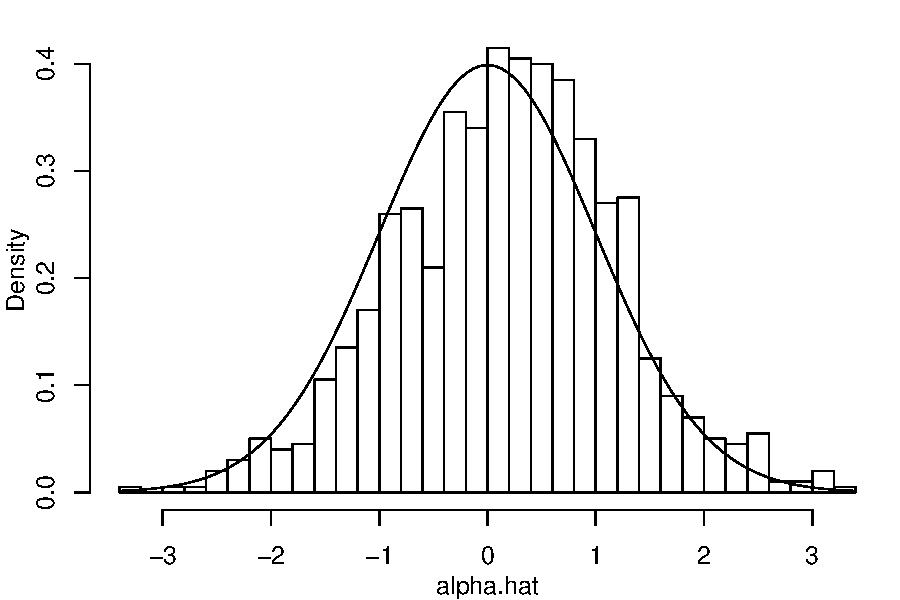
\includegraphics{HDM-HC}
\end{center}
\caption{Histogram of the centered and rescaled estimated values for the treatment effect $\alpha$; standard normal distribution is given by the solid line.}
\end{figure}

For the case that there is not only one but several treatment variables \texttt{d} two functions are provided: \texttt{HC.lasso.wrap} and \texttt{HC.lasso.mult}. The first one takes \texttt{x} and \texttt{y} as arguments and additionally an \texttt{index} which denotes the column number of variables in \texttt{x} which should be handled as treatment variable. For each case then the function \texttt{HC.lasso} is applied with \texttt{d} selected accordingly. The function \texttt{HC.lasso.mult} takes as arguments \texttt{x,y} and \texttt{d} where the treatment can now be multivariate.


\subsection{Estimation and Inference on Structural Effects with High-dimensional Instruments}
In many empirical applications there are many potential instrumental variables and the researcher has to make a decision which one to include. Selection of instrumental variables in a high-dimensional setting has been analysed in \cite{BCCH12}. The function \texttt{IV.lasso} implements this procedure what we will demonstrate with an example.
First, we simulate data with the function \texttt{DGP.IV} which implements the data generating process used in \cite{BCCH12}. Strictly speaking, the function implements the cut-off design with \texttt{pz} the number of variables with non-zero coefficients. A detailed description is given in \cite{BCCH12} and in the help for the function. An example shows how to estimate the model:

\begin{Schunk}
\begin{Sinput}
> data <- DGP.IV(n=250, p=100, pnz=5, Fstat=180, 
+                control=list(s2e=1, Cev=.6, s2z=1, szz=.5, pi1=1, alpha=1))
>   y <- data$y
>   d <- data$X
>   z <- data$Z
>   x <- NULL
>   l <- IV.lasso(x,d,y,z, post=TRUE, intercept=TRUE, normalize=FALSE)
>   l$coefficients
\end{Sinput}
\begin{Soutput}
       [,1]
d1 1.015131
\end{Soutput}
\begin{Sinput}
>   l$vcov
\end{Sinput}
\begin{Soutput}
           d1
d1 0.01115212
\end{Soutput}
\end{Schunk}
\texttt{x} denotes the control variables, \texttt{z} the instrumental variables, \texttt{d} the endogenous outcome variables, and \texttt{y} the outcome or dependent variable. Again, arguments, additionally to the \texttt{post}-option can be passed to the function \texttt{lasso} via the $\ldots$-mechanism.

Again, we demonstrate the asymptotic properties of the estimator in a small simulation study:

\begin{Schunk}
\begin{Sinput}
> R <- 1000
> result <- matrix(NA, ncol=2, nrow=R)
> for (i in 1:R) {  
+   data <- DGP.IV(n=250, p=100, pnz=5, Fstat=180, 
+                  control=list(s2e=1, Cev=.6, s2z=1, szz=.5, pi1=1, alpha=1))
+   l <- try(IV.lasso(NULL,data$X,data$y,data$Z, post=TRUE, intercept=TRUE, normalize=FALSE))
+   if (class(l)=="error") {
+     next
+   } else {
+     result[i,1] <- l$coef[1]
+     result[i,2] <- l$vcov[1,1]
+   }
+ }
\end{Sinput}
\end{Schunk}

Finally, we plot the centered and rescaled estimated values which should approximately normally distributed as shown in Figure \ref{IV}.

\begin{figure}[h!]
\begin{center}
\label{IV}
\begin{Schunk}
\begin{Sinput}
> alpha.hat <- (result[,1]-1)/sqrt(result[,2])
> hist(alpha.hat, breaks=25, freq=F, main="")
> curve(dnorm(x), add=TRUE)
\end{Sinput}
\end{Schunk}
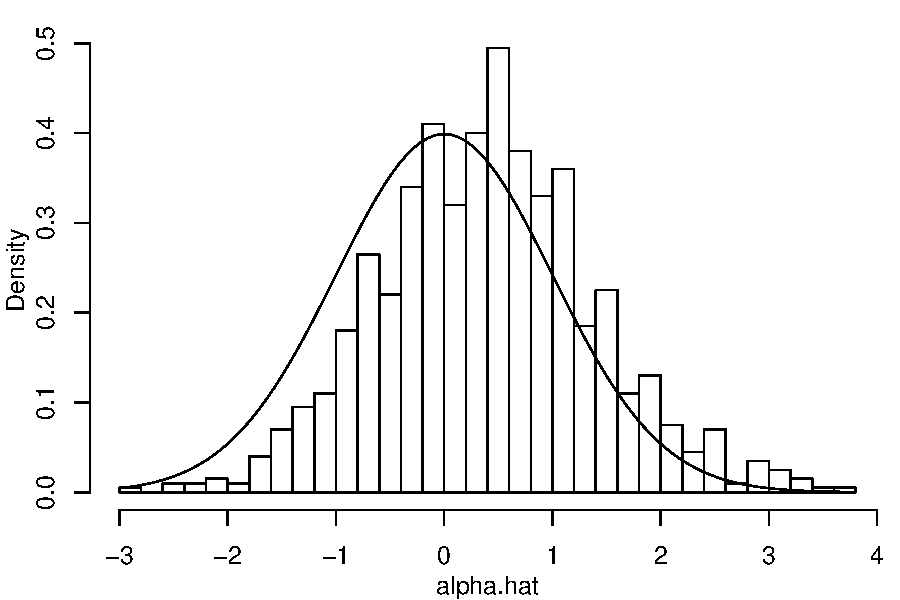
\includegraphics{HDM-IV}
\end{center}
\caption{Histogram of the centered and rescaled estimated values for the treatment effect $\alpha$; standard normal distribution is given by the solid line.}
\end{figure}

\subsection{Estimation and Inference on Structural Effects with High-dimensional Controls and Instruments}
Finally, in this section we combine the settings in the two previous sections to estimation in a setting with many controls and many instruments. A formal analysis is provided in \cite{CHS:2015}. The method relying on double selection is implemented in the function \texttt{HCHIV.lasso}.
To demonstrate how to apply this function we first simulate a data set with a dgp as described in  \cite{CHS:2015} and then estimate it:

\begin{Schunk}
\begin{Sinput}
>  data <- DGP.HCHIV()
>   y <- data$y
>   d <- data$d
>   x <- data$X
>   z <- data$Z
>   res <- HCHIV.lasso(x,z,y,d)
>   res
\end{Sinput}
\begin{Soutput}
$coefficient
         [,1]
[1,] 0.989623

$se
           [,1]
[1,] 0.08910734
\end{Soutput}
\end{Schunk}

A simulation example is as following

\begin{Schunk}
\begin{Sinput}
> R <- 1000
> result <- matrix(NA, ncol=2, nrow=R)
> for (i in 1:R) {
+   data <- DGP.HCHIV()
+   res <- try(HCHIV.lasso(data$X,data$Z,data$y,data$d))
+   if (class(res)=="error") {
+     next
+   } else {
+   result[i,1] <- res[[1]]
+   result[i,2] <- res[[2]]
+   }
+ }
\end{Sinput}
\end{Schunk}
with the empirical distribution of the centered and normalized estimates given in Figure \ref{HCIV}.
\begin{figure}[h!]
\begin{center}
\label{HCIV}
\begin{Schunk}
\begin{Sinput}
> alpha.hat <- (result[,1]-1)/result[,2]
> hist(alpha.hat, breaks=25, freq=F, main="")
> curve(dnorm(x), add=TRUE)
\end{Sinput}
\end{Schunk}
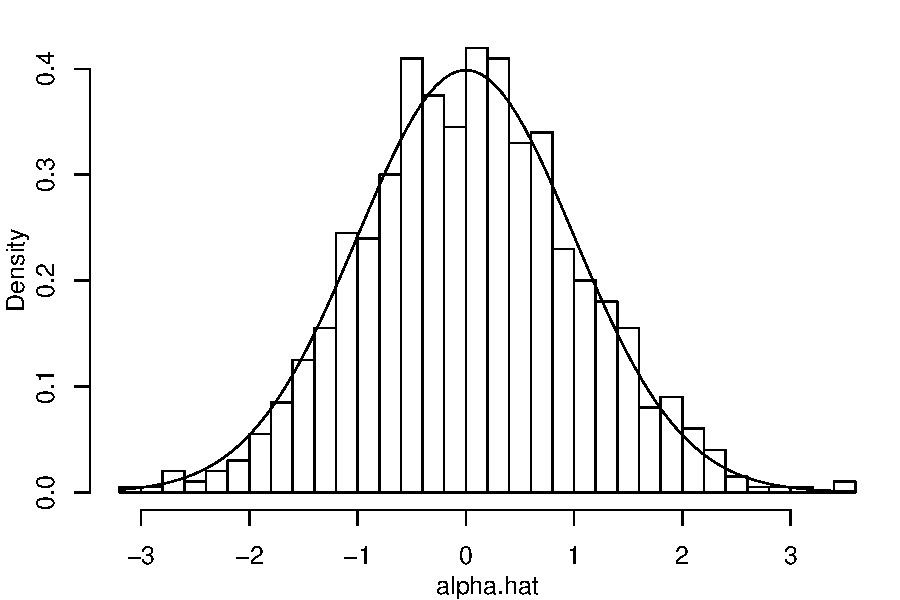
\includegraphics{HDM-HCHIV}
\end{center}
\caption{Histogram of the centered and rescaled estimated values for the treatment effect $\alpha$; standard normal distribution is given by the solid line.}
\end{figure}

\section{Program Evaluation}
We also provide functions for estimation and inference on policy relevant treatment effects in a high-dimensional setting. The ideas and theoretical results are given in \cite{BCFH:Policy}. The function \code{ProgEval} estimates the local average treatment effect (LATE) and the local average treatment effect of the treated (LATE-T). Moreover, local quantile treatment effects (LQTE) and the LQTE of the treated (LQTE-T) at user-specified quantiles are estimated. For calculation of the standard errors bootstrap methods can be employed, namely, the normal, wild and Bayes bootstrap. The output of a function call to \code{ProgEval} can be plotted with the function \code{LQplot}.
We demonstrate the usage of the functions by estimating the effect of 401(k) participation on accumulated assets. The data set is contained in the package and can be accessed in the following way:
\begin{Schunk}
\begin{Sinput}
> data(pension)
> help(pension)
\end{Sinput}
\end{Schunk}

\begin{Schunk}
\begin{Sinput}
> help(pension)
\end{Sinput}
\end{Schunk}

As 401(k) participation -- the treatment variable -- is presumably endogenous, we use 401(k) eligibility as an instrument. For illustration purpose we construct a matrix of control variables containing selected socio-economic variables where the variables age, income, family size and education are transformed by high-order orthogonal polynomial. The outcome variable (e.g. total wealth) is denoted by y, the treatment variable by d, the instrument by z. The analysis of treatment effects can be done as shown below. Moreover, the LQTE and LQTE-T can also be plotted.

\begin{Schunk}
\begin{Soutput}
[1] "No variables selected!"
[1] "No variables selected!"
[1] "No variables selected!"
[1] "No variables selected!"
[1] "No variables selected!"
[1] "No variables selected!"
[1] "No variables selected!"
[1] "No variables selected!"
[1] "No variables selected!"
[1] "No variables selected!"
[1] "No variables selected!"
[1] "No variables selected!"
[1] "No variables selected!"
[1] "No variables selected!"
[1] "No variables selected!"
[1] "No variables selected!"
[1] "No variables selected!"
[1] "No variables selected!"
[1] "No variables selected!"
[1] "No variables selected!"
\end{Soutput}
\end{Schunk}
\begin{Schunk}
\begin{Sinput}
> str(effects)
\end{Sinput}
\begin{Soutput}
List of 6
 $ LATE     :List of 4
  ..$ se        : num [1, 1] 1645
  ..$ late      : num 11584
  ..$ individual: num [1:9915, 1] -7380 -99494 141649 24635 34524 ...
  ..$ boot.se   : num 1556
 $ LATT     :List of 4
  ..$ se        : num [1, 1] 2193
  ..$ latt      : num 16692
  ..$ individual: num [1:9915, 1] -690 -103527 157645 25637 49202 ...
  ..$ boot.se   : num 2309
 $ LQTE     :List of 3
  ..$ lqte: num [1:84] NA -667 188 883 961 ...
  ..$ se  : num [1:84] NA NA NA NA NA ...
  ..$ t   : Named num 5.28
  .. ..- attr(*, "names")= chr "95%"
 $ LQTT     :List of 3
  ..$ lqtt: num [1:84] NA NA 4860 4118 3705 ...
  ..$ se  : num [1:84] NA NA NA NA 804 ...
  ..$ t   : Named num 3.79
  .. ..- attr(*, "names")= chr "95%"
 $ bootstrap: chr "wild"
 $ tau      : int [1:84] 1 2 3 4 5 6 7 8 9 10 ...
\end{Soutput}
\end{Schunk}
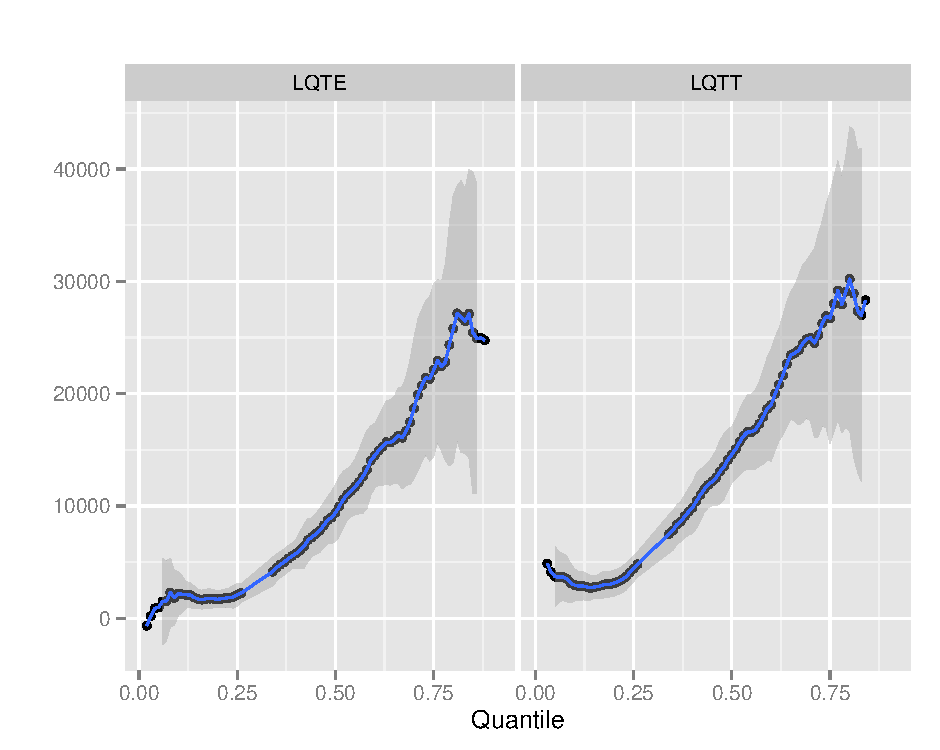
\includegraphics{Program}
\end{center}
\caption{Local Quantile Treatment Effect (LQTE) and the corresponding effect of the Treated (LQTT) at selected quantiles}
\end{figure}

\section{Related \R packages}
\R already contains many very useful packages for high-dimensional problems. In this section we review some packages which are related to our package but without any claim to be complete as currently the field is evolving very fast. A good starting point for the interested reader is the CRAN Task View \texttt{Machine Learning & Statistical Learning} which points to many methods available as \R packages.

Two classical and very established packages to estimate LASSO Regression are \Rpackage{glmnet} (\cite{glmnet})and \Rpackage{lars} (\cite{lars}).  \Rpackage{lars} fit Least Angle Regression, Lasso and Infinitesimal Forward Stagewise regression models, but does not allow data depenent penalties. \Rpackage{glmnet} fits generalized linear models via penalized maximum likelihood. The regularization path is computed for the elastic net penalty (elastic net contains LASSO as a special case) at a grid of values. A separate penalty factors can be applied to each coefficient. The \Rpackage{grplasso} (\cite{grplasso}) estimates group LASSO models. A very recent \R package is \Rpackage{flare} (\cite{flare}) which implements a family of novel regression methods (Lasso, Dantzig Selector, LAD Lasso, SQRT Lasso, Lq Lasso) and their extensions to sparse precision matrix estimation (TIGER and CLIME using L1) in high dimensions.


\section{Some Tips and Tricks}
This section conatains some practical tips and tricks when using the package.

\begin{itemize}
 \item Most functions require the outcome variable y, the control variables x, instruments z, or treatment variable d, as vector or matrix. Data.frames are not allowed, but can easily forced to vector/matrix.
 \item When transforming / coding factor variables to several binary variables, the function \code{model.matrix} might be useful. It also returns a matrix as required.
 \item The functions  \code{bs} from the \Rpackage{splines} and \code{poly} are useful for transforming variables into splines or orthogonal polynomials.
 \item The methods \code{predict} which are provided with the function should be used together with the argument \code{newdata}, even if prediction should be done on the passed object.
\end{itemize}

\section{Conclusion}

An introduction to some of the capabilities of the \R package \texttt{hdm}
package has been given with some examples describing its basic functionality. Inevitably, new applications will
demand new features and, as the project is in its initial phase, unforseen bugs will show up. In either case comments and suggestions of users are highly appreciated. It is intended to update the documentation (including this vignette) and the package periodcally. The most current version of the \R package and its accompanying vignette will be made available at the homepage of the maintainer and \texttt{cran.r-project.org}. See the \R command \texttt{vignette()} for details on how to find
and view vignettes from within \R.



\footnotesize
\bibliographystyle{aea}
\bibliography{mybib}
\end{document}
